\documentclass{article}
\usepackage{fancyhdr}
\usepackage{amsmath,amssymb}
\usepackage{geometry}
\usepackage{datetime}
\usepackage{enumerate}
\usepackage{graphicx}

%Insert page formatting here
\hoffset = -.5in
\voffset = -0.375in
\textwidth = 7in
\textheight = 10in
\headheight = 24pt

\pagestyle{fancy}

\rhead{Peter Olson\\Student ID: $441666$}
\lhead{Math 3200\\Homework 1}
\chead{\today}
\cfoot{}

\renewcommand{\labelitemi}{$\diamond$}
\renewcommand{\implies}{\rightarrow}
\newcommand{\widespace}{\qquad \qquad \;}
\newcommand{\tret}{\\ \hline}
\newcommand{\fh}{\tfrac{1}{2}}
\newcommand{\deriv}[2]{\frac{d #1}{d #2}}
\newcommand{\pderiv}[2]{\frac{\delta #1}{\delta #2}}
\newcommand{\vr}{\vec{r}}
\newcommand{\at}{\text{ at }}

\begin{document}
\section*{Question 5}
\begin{enumerate}[a)]
	\item Report the five number summaries of jumping distance.
	
	\begin{tabular}{|c|c|c|c|c|}
		\hline 
		Min & 1st Quartile & Median & 3rd Quartile & Max \\ 
		\hline 
		13.71 & 15.35 & 16.43 & 17.62 & 18.17 \\ 
		\hline 
	\end{tabular} \vspace{1em}

	\item Please construct a scatter plot with a regression line.\\
	\begin{center}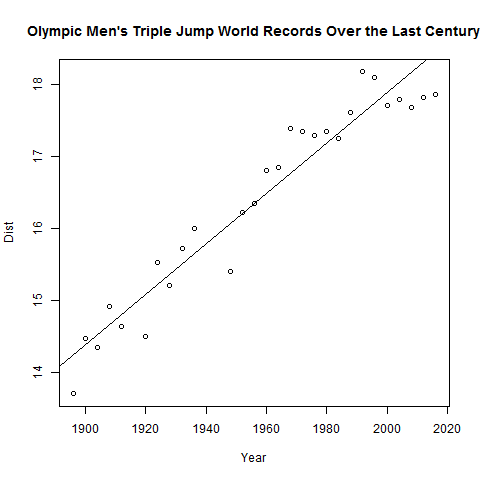
\includegraphics[width=4in]{Q5.png}\end{center}
	\item What are the covariance and correlation between "year" and "distance"?
	
	The covariance and correlation between the year and the distance are 48.477354 and 0.961747 respectively. Having a large positive covariance suggests that, as the years wear on, there is a demonstrable improvement in the distance that the jumpers can travel. Having a correlation that's very close to one suggests that time and distance, here, are tightly coupled. Note, though, that there's nothing to be said as to \emph{why} these two variables are correlated, and a strong numerical correlation is hardly enough to prove a causational relationship between the two.
	
\end{enumerate}
\newpage
	\subsection*{R Source}
\begin{verbatim}
#      Problem 5 - R Code
# =============================
#     Author - Peter Olson
#       Date - 2017-01-27
#   Filename - MensJump.R
# =============================

# Prep dataframe
m <- read.table("MenTripleJumpOlympics.txt", header=TRUE)

# Part A
print(summary(m$Dist))			# Show the summary of the distance

# Part B
plot(m)					# Create the plot
abline(lm(Dist~Year, data=m))		# Add linreg line

# Part C					# Use sprintf to prep and show descriptors
print(sprintf("The covariance between the year and the distance is: %f", cov(m$Year, m$Dist)))
print(sprintf("The correlation between the year and the distance is: %f", cor(m$Year, m$Dist)))

# Clean up variables
rm(m)						# de-clutter workspace
\end{verbatim}
\subsection*{Console Output}
\begin{verbatim}
> source("MensJump.R")
Min.   1st Qu.  Median    Mean  3rd Qu.    Max. 
13.71   15.35    16.83   16.43   17.62    18.17 
[1] "The covariance between the year and the distance is: 48.477354"
[1] "The correlation between the year and the distance is: 0.961747"
\end{verbatim}

\end{document}